\Diskussionspunkt{Themen sind technische Umsetzung, Zusammenarbeit mit Dritten, Termine, Ressourcen, }
\subsection{Risikoliste}
Für die Risikoanalyse haben wir eine Liste der möglichen  Risiken erstellt. Als Grundlage verwendeten wir das Risikolexikon aus dem Buch \flqq IT-Risikomanagment leben!\frqq ~\cite{AhrendtsFabian2008Il:w}. 
Für jedes Risiko haben wir die Eintretenswahrscheinlichkeit und das Ausmass abgeschätzt. Gegenüber den herkömmlichen Risikobeurteilungen, haben wir allerdings die Auswirkungen auf Kosten und Terminverzug weggelassen, da sie in unserem Projekt nicht relevant sind und uns auf den Stundenaufwand und den Funktionsumfang beschränkt. Um die Auswirkung der einzelen Risiken abschätzen zu können, haben wir eine Punkteskala mit entsprechenden Kriterien erstellt, wie in Tabelle \ref{tab:auswirkung} aufgeführt. Die komplette Risikoliste\ref{img:risikoliste} befindet sich auf Seite \pageref{img:risikoliste}.

\vspace{5mm} %5mm vertical space

\begin{table}[]
\centering
\label{tab:auswirkung}
\begin{tabular}{rl}
Wert	[-]	& 	Auswirkung bezüglich Umfang \\
\hline
10	&	Gesamter Block nicht funktionsfähig \\
8	&	Einzelne Funktion nicht umgesetzt  \\
6	&	Bemerkbar, keine Funktionseinbusse \\
4	&	von eingeschränkter Benutzergruppe bemerkbar \\
2	&	von Kunden nicht bemerkbar
\end{tabular}
\end{table}

\subsection{Risikomatrix}
Die Risikomatrix zeigt auf grafische Weise wie kritisch die einzelnen Risiken aus der Risikoliste\ref{img:risikoliste}  sind. Mindestens vier davon sind als hoch eingestuft und müssen im Rahmen der Bachelor-Arbeit reduziert werden.

% Abbildung der Risikomatrix
\begin{figure}[htbp]
	\centering
	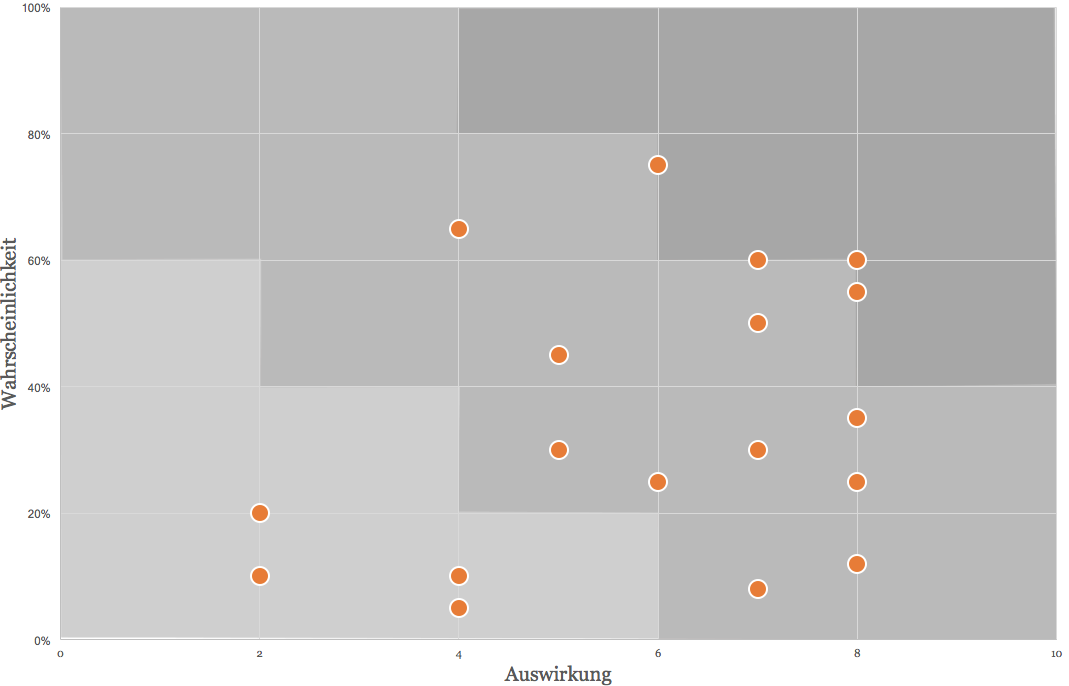
\includegraphics[width=0.9\linewidth]{img/risikomatrix} 
	\caption{Risikomatrix}
	\label{img:risikomatrix}
\end{figure}


% Abbildung der Risikoliste (A3)
\newpage
\clearpage
\pagebreak
\afterpage{ % Insert after the current page
\clearpage
\KOMAoptions{paper=a3, paper=landscape} 
\recalctypearea

\begin{figure}[htbp]
	\centering
	\includegraphics[width=1.1\linewidth]{img/risikoliste} % ab heigth = 0.6 auf eigener Seite!
	\caption{Risikoliste}
	\label{img:risikoliste}
\end{figure}


% PDF einbinden
%\includepdf[pages=1,  width=\textwidth, height=\textheight]{risikoliste.pdf} 
\clearpage
\KOMAoptions{paper=A4,pagesize}
\recalctypearea
}







